\section{Introduction} 
Au cours de ce chapitre, nous aborderons plusieurs points essentiels. Dans un premier temps, nous présenterons le cadre général du projet ainsi que la société au sein de laquelle il a été réalisé. Ensuite, nous effectuerons une analyse de l’existant accompagnée d’une étude critique des méthodes de travail actuelles. Enfin, nous exposerons la méthodologie de développement adoptée pour la réalisation de ce projet. 

\section{Cadre du projet} 
Le présent travail s’inscrit dans le cadre de mon projet de fin d’études, réalisé en vue de l’obtention du Diplôme National d’Ingénieur en Génie Logiciel à l’IT Business School de Nabeul.

En collaboration avec la société AfterCode, ce projet intitulé \textbf{« Conception et développement d’une plateforme microservices dédiée aux animaux domestiques »}, baptisé \textbf{AniHub}, a pour objectif de concevoir et mettre en place une plateforme d’animalerie en ligne en Tunisie. Cette solution vise à moderniser, structurer et faciliter la gestion du secteur des animaux domestiques. 

\section{Organisme d’accueil}

AfterCode est une agence spécialisée dans le développement web et mobilee, fondée en 2020 . Elle propose une large gamme de services digitaux, allant de la conception de sites web vitrines et e-commerce à la création de solutions web et mobiles sur mesure, en passant par le community management, le référencement naturel (SEO) et l’hébergement web.

L’objectif principal de l’agence est d’accompagner les entreprises dans leur transformation digitale, d’améliorer leur visibilité en ligne, d’augmenter leur trafic et d’optimiser leur retour sur investissement. Pour atteindre ces objectifs, AfterCode s’appuie sur une équipe de développeurs passionnés et expérimentés, travaillant en étroite collaboration avec les clients afin de fournir des solutions innovantes et adaptées à leurs besoins.
\newpage

La figure \ref{fig:aftercode_logo} présente le logo de la société AfterCode : 

\begin{figure}[H]%
    \center%
    
\includegraphics[width=4cm,height=3cm]{images/aftercode.png}%
    \caption{Logo AfterCode \cite{aftercode2020}}%
    \label{fig:aftercode_logo}
\end{figure}

\vspace{0.5cm}

Les services proposés par AfterCode se déclinent comme suit :

\begin{itemize}
\item \textbf{Applications web :} conception et développement de solutions web sur mesure, allant des plateformes métiers aux applications de gestion, afin de répondre précisément aux besoins fonctionnels des clients. Ces solutions sont pensées pour être évolutives, performantes et optimisées en termes de coût et de qualité.

\item \textbf{Applications mobiles :} développement d’applications Android et iOS intuitives, performantes et adaptées aux usages modernes. L’objectif est de garantir une expérience utilisateur fluide, une interface ergonomique et une compatibilité optimale avec les différents appareils mobiles.

\item \textbf{Sites e-commerce :} création de boutiques en ligne complètes intégrant la gestion des produits, des commandes et des paiements sécurisés. Ces solutions visent à renforcer la présence digitale des entreprises, à améliorer leur visibilité et à maximiser leurs ventes.

\item \textbf{Community management :} gestion et animation des réseaux sociaux des clients à travers la création de contenu, la planification de publications et le suivi des interactions, dans le but de renforcer l’image de marque et d’améliorer l’engagement du public.

\item \textbf{Formations :} mise en place de programmes de formation en développement web et mobile, combinant théorie et pratique, afin de permettre aux apprenants d’acquérir des compétences concrètes et directement exploitables dans le milieu professionnel.

\item \textbf{Référencement web (SEO) :} optimisation technique et éditoriale des sites web afin d’améliorer leur visibilité sur les moteurs de recherche, d’augmenter le trafic organique et d’assurer un meilleur positionnement face à la concurrence.

\item \textbf{Hébergement web :} fourniture de solutions d’hébergement sécurisées et fiables, incluant la gestion des serveurs, des bases de données et des noms de domaine, afin de garantir la disponibilité continue et la stabilité des sites web des clients.
\end{itemize}


\section{Étude de l’existant}

Dans le cadre de ce projet, une étude approfondie du marché a été menée afin d’analyser les solutions existantes proposant des services similaires. Cette analyse comparative a permis d’identifier les limites et les insuffisances des plateformes concurrentes.

Sur cette base, nous avons défini un ensemble de fonctionnalités améliorées et innovantes, dans le but de proposer une solution plus performante et mieux adaptée aux besoins des utilisateurs. 

\subsection{Panorama du marché des animaux domestiques en Tunisie} 
En Tunisie, le secteur des animaux domestiques reste peu structuré et manque de plateformes C2C dédiées. Les prestataires de services, tels que les dresseurs, toiletteurs, pet-sitters et vétérinaires, ne disposent pas d’espaces adaptés pour promouvoir leurs services en ligne. De plus, l’adoption et la vente d’animaux entre particuliers restent peu organisées et se font principalement au marché de Moncef Bey.

Face à ce manque de centralisation et de digitalisation, nous avons proposé \textbf{AniHub}, une plateforme C2C permettant de regrouper les services, l’adoption et la mise en relation entre particuliers autour des animaux domestiques en Tunisie . 
\subsection{Critique de l’existant} 
Dans cette section, nous présenterons les solutions existantes en Tunisie ainsi que leurs principaux atouts et limites. 
\subsubsection{Les animaleries en Tunisie}

En Tunisie, plusieurs animaleries en ligne, comme AnimalZone, Mypets et Z’animo, proposent des produits et accessoires pour animaux selon un modèle B2C, sans interaction entre particuliers.

Les figures \ref{fig:mypets}, \ref{fig:animalzone} et \ref{fig:zanimo} présentent les logos de ces plateformes :

\begin{figure}[ht]
\centering

\makebox[\textwidth][c]{
\begin{minipage}[b]{0.3\linewidth}
\centering

\includegraphics[width=0.8\linewidth]{images/mypets.png}
\caption{logo Mypets \cite{mypets2026}}
\label{fig:mypets}
\end{minipage}
\hfill

\begin{minipage}[b]{0.3\linewidth}
\centering
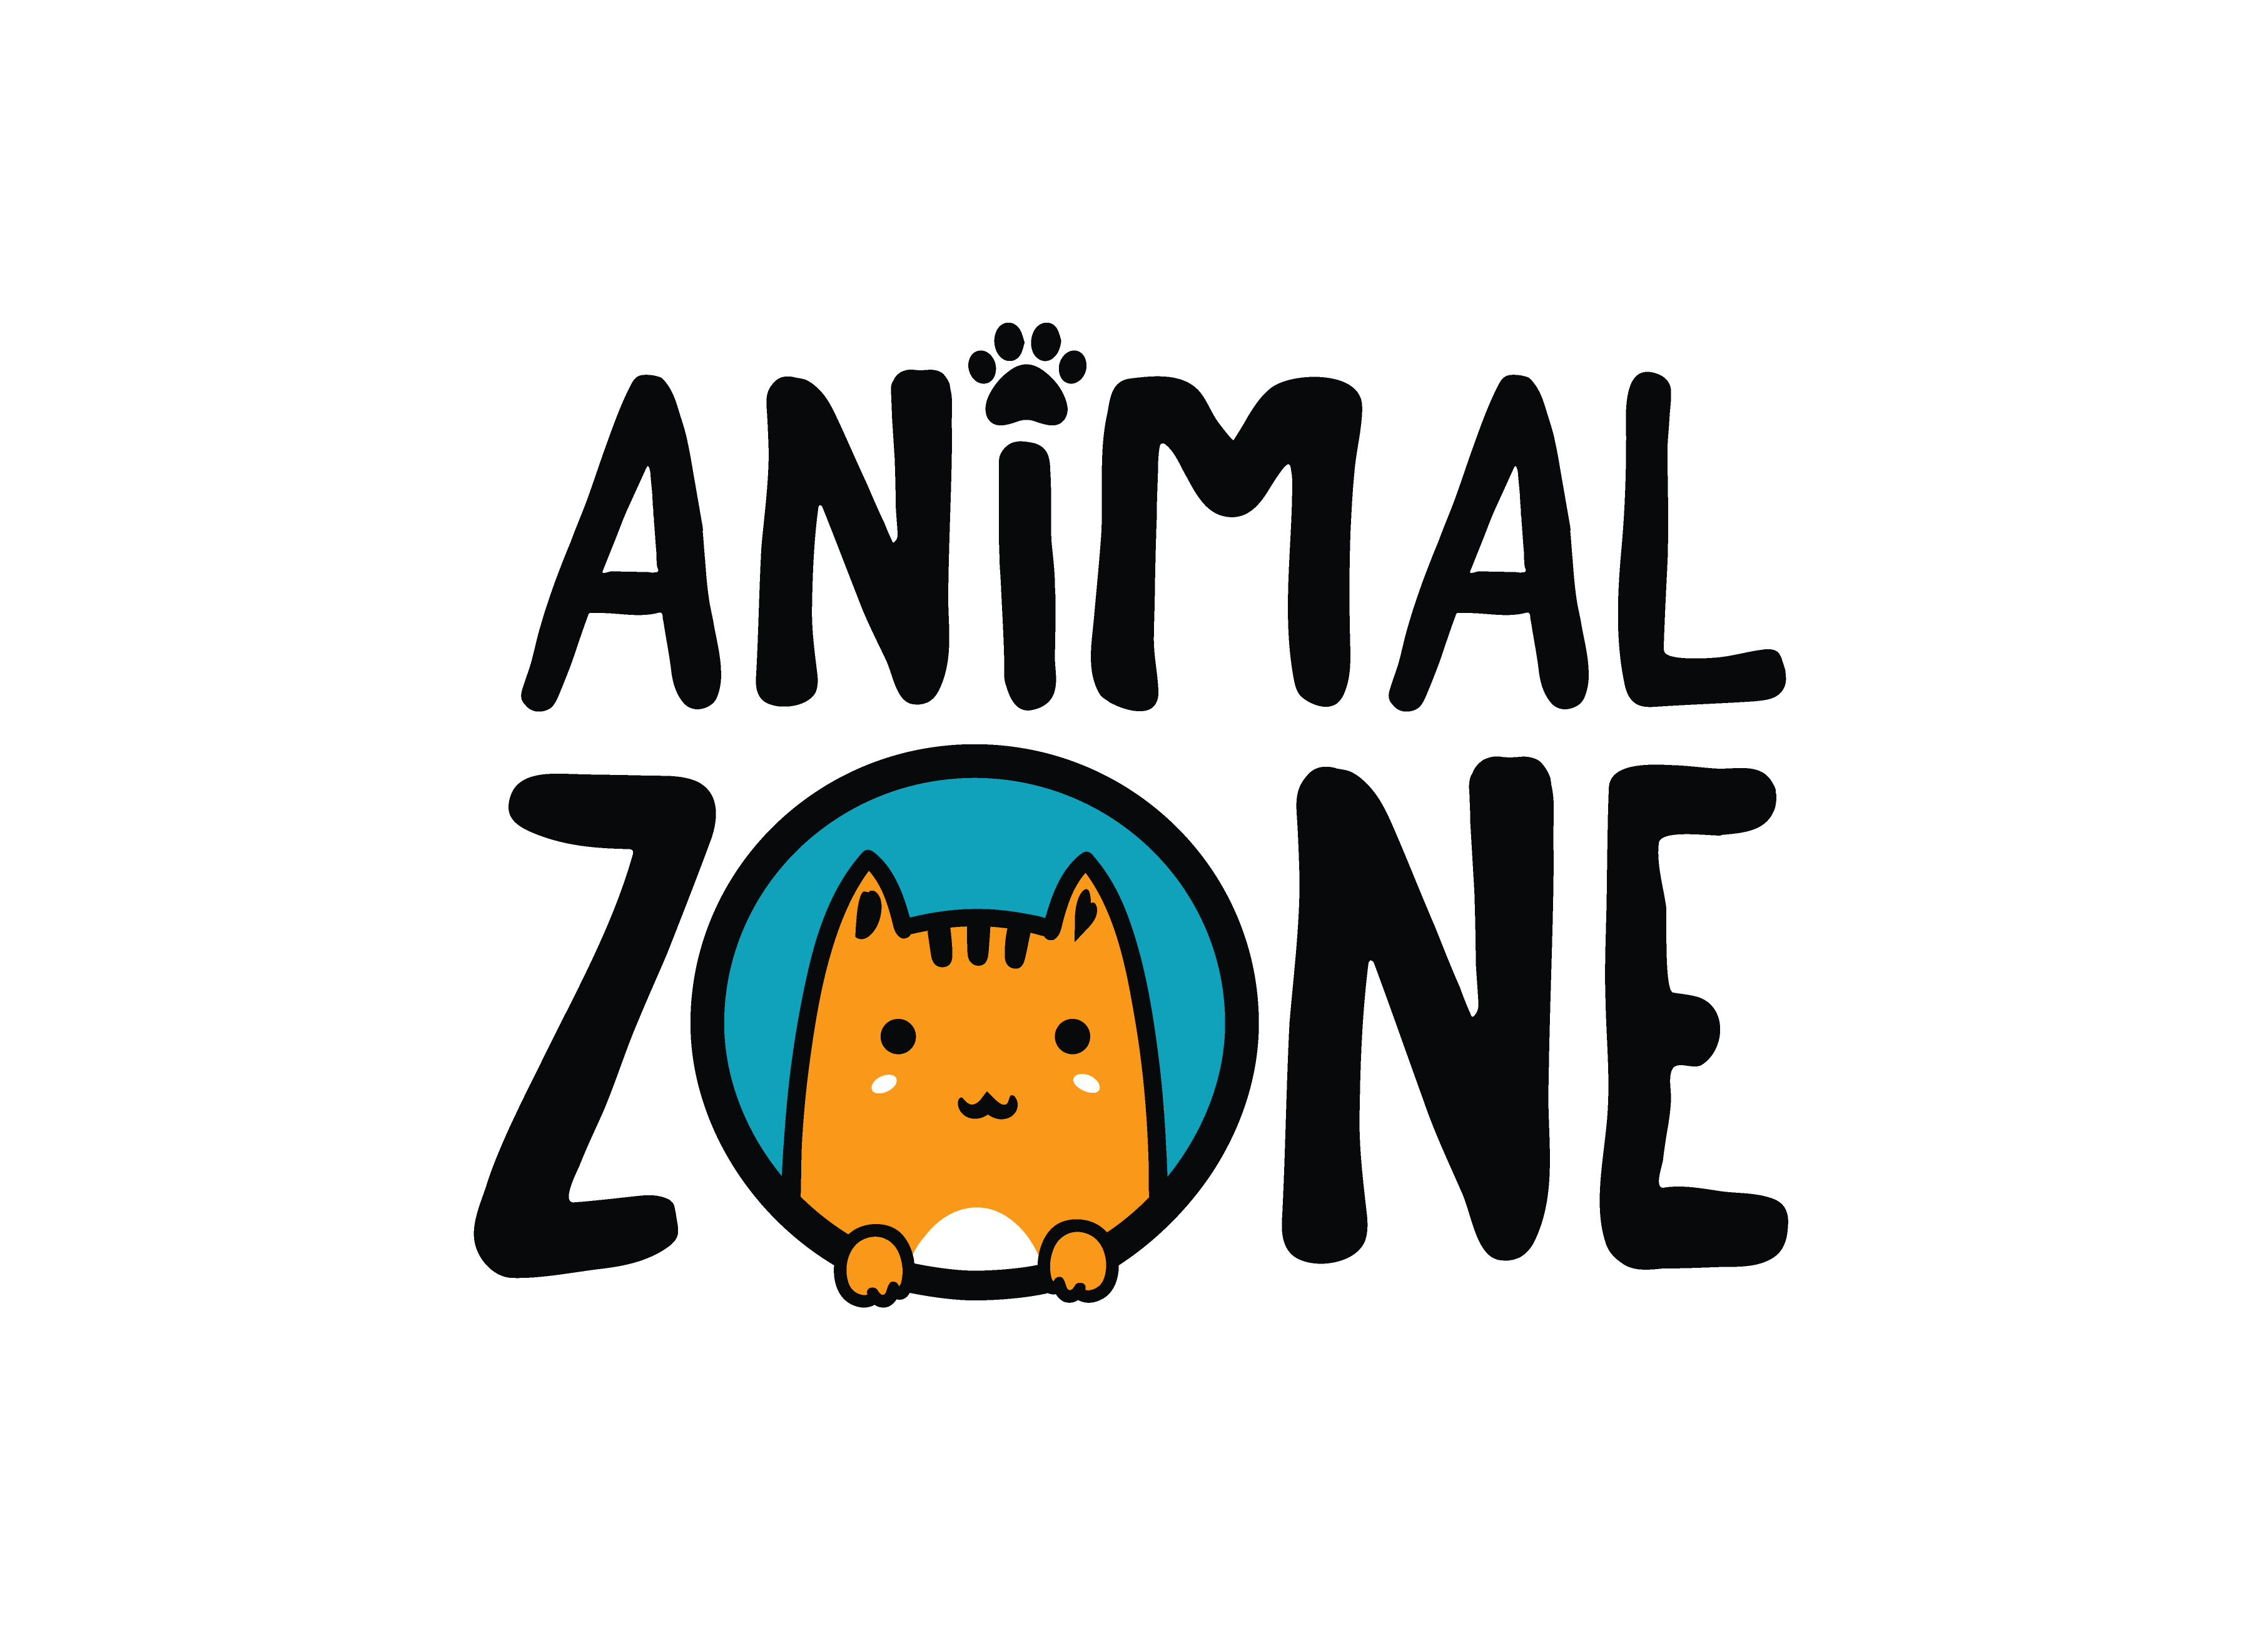
\includegraphics[width=0.8\linewidth]{images/animalzone.png}
\caption{logo AnimalZone \cite{animalzone2026}}
\label{fig:animalzone}
\end{minipage}
\hfill

\begin{minipage}[b]{0.3\linewidth}
\centering

\includegraphics[width=0.8\linewidth]{images/zanimo.png}
\caption{logo Z'animo \cite{zanimo2026}}
\label{fig:zanimo}
\end{minipage}
}

\end{figure}

\begin{itemize}
\item \textbf{Points forts :}
\begin{itemize}
\item Large variété de produits proposés
\item Interfaces simples, intuitives et faciles à utiliser
\end{itemize}

\item \textbf{Points faibles :}
\begin{itemize}
\item Absence d’un système d’évaluation et de notation des produits
\item Absence d’un modèle C2C (Consumer-to-Consumer) permettant aux particuliers de publier et de commercialiser leurs propres articles
\item Offre principalement limitée à la commercialisation de produits et, dans certains cas, d’animaux, sans intégration de services associés (toilettage, garde, dressage) ni de fonctionnalités dédiées à l’adoption
\end{itemize}
\end{itemize}
\subsubsection{Réseaux sociaux (Facebook et Instagram)}

En Tunisie, les particuliers utilisent principalement Facebook, Instagram et les groupes spécialisés pour la vente et l’adoption d’animaux. Cependant, ces échanges restent peu structurés et faiblement encadrés.

Les figures \ref{fig:instagram} et \ref{fig:facebook} présentent les logos de Facebook et Instagram. 
\begin{figure}[ht]
\centering

\begin{minipage}[b]{0.45\linewidth}
\centering

\includegraphics[width=0.2\linewidth]{images/instagram.png}
\caption{Logo Instagram \cite{instagram2026}}
\label{fig:instagram}
\end{minipage}
\hfill
\begin{minipage}[b]{0.45\linewidth}
\centering

\includegraphics[width=0.2\linewidth]{images/facebook logo.png}
\caption{Logo Facebook \cite{facebook2026}}
\label{fig:facebook}
\end{minipage}

\end{figure} 


\begin{itemize}
\item \textbf{Points forts :}
\begin{itemize}
\item Large audience : Accès à des millions d’utilisateurs en Tunisie, offrant ainsi une forte visibilité des annonces en très peu de temps.
\item Gratuité et simplicité : Publication simple et rapide, sans frais associés pour la mise en ligne des annonces.
\item  Rapidité de mise en relation : Contact direct via Messenger ou commentaires
\end{itemize}

\item \textbf{Points faibles :}
\begin{itemize}
\item Absence de structure (Pas de filtres , Annonces mélangées et non organisées ) 
\item Aucune vérification des animaux
\item Manque de sécurité et d’arnaques (Faux profils fréquents , Risque de fraude ou mauvaise intention )
\end{itemize}
\end{itemize} 

\subsubsection{Les sites d’annonces généralistes} 
En Tunisie, les particuliers utilisent également des sites d’annonces généralistes comme Tayara et Afariat pour publier des annonces de vente d’animaux domestiques et atteindre un public plus large.

Les figures \ref{fig:tayara}, \ref{fig:afariat} et \ref{fig:bazarafrique} présentent les logos de ces plateformes : 
\begin{figure}[ht]
\centering
\begin{minipage}[b]{0.3\linewidth}
\centering
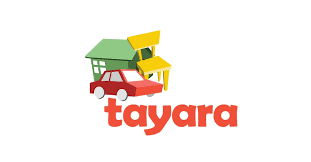
\includegraphics[width=\linewidth]{images/tayara.png}
\caption{logo Tayara \cite{tayara2026}}
\label{fig:tayara}
\end{minipage}
\hfill
\begin{minipage}[b]{0.3\linewidth}
\centering
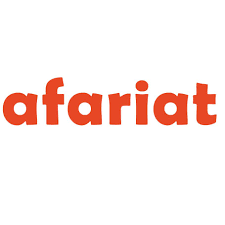
\includegraphics[width=0.7\linewidth]{images/afariat.png}
\caption{logo Afariat   \cite{afariat2026}}
\label{fig:afariat}
\end{minipage}
\hfill
\begin{minipage}[b]{0.3\linewidth}
\centering

\includegraphics[width=0.8\linewidth]{images/bazarafrique.jpg}
\caption{logo bazarafrique \cite{bazarafrique2026}}
\label{fig:bazarafrique}
\end{minipage}
\end{figure} 


\begin{itemize}
\item \textbf{Points forts :}
\begin{itemize}
\item Forte visibilité des annonces
\item Accessibilité facile 
\item  Gratuité ou faible coût
\end{itemize}

\item \textbf{Points faibles :}
\begin{itemize}
\item Mauvaise expérience utilisateur pour les animaux : Recherche difficile et peu optimisée et pas de fonctionnalités dédiées (matching, wishlist, historique)
\item Manque de confiance et de contrôle : Aucune vérification des vendeurs ou des animaux
\item Absence de spécialisation animale : Les animaux sont mélangés avec d’autres catégories (voitures, immobilier…)
\end{itemize}
\end{itemize}  

\section{Solution proposée}  
\subsection{Présentation de notre solution AniHub}

La figure ci-dessous présente le squelette général de la plateforme \textbf{AniHub}. Elle met en évidence l’architecture fonctionnelle de la solution ainsi que ses principaux modules. Cette organisation permet de comprendre clairement la structure globale de la plateforme, la logique d’interaction entre ses composants et la répartition détaillée de ses fonctionnalités, offrant ainsi une vision globale et cohérente de son fonctionnement.

\begin{figure}[H]
    \centering
    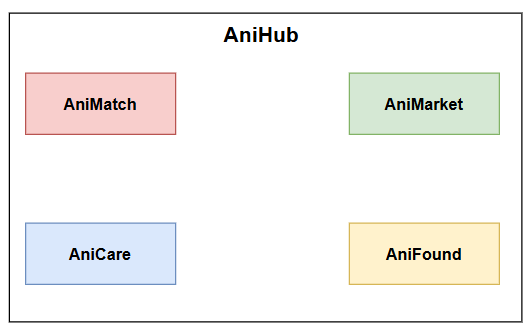
\includegraphics[width=0.7\textwidth]{images/squelette.png}
    \caption{Squelette fonctionnel de la plateforme AniHub}
    \label{fig:anihub-squelette}
\end{figure}

\noindent La plateforme AniHub s’articule autour de quatre modules principaux :

\begin{itemize}
    \item \textbf{AniMatch} : ce module est dédié à la mise en relation des propriétaires d’animaux dans un cadre structuré et sécurisé. Il facilite d’une part l’accouplement responsable des animaux en tenant compte de critères de compatibilité, et d’autre part l’adoption en permettant aux animaux de trouver de nouveaux foyers adaptés à leurs besoins, tout en favorisant une démarche responsable et encadrée.

    \item \textbf{AniMarket} : ce module constitue une marketplace spécialisée dans le domaine animalier. Il permet non seulement l’achat et la vente d’animaux domestiques, mais aussi la publication, la consultation et la gestion d’annonces relatives aux produits, accessoires et équipements destinés aux animaux, offrant ainsi un espace commercial complet et centralisé.

    \item \textbf{AniCare} : ce module regroupe un ensemble de services dédiés au bien-être et à la santé animale. Il met en relation les propriétaires avec des professionnels qualifiés tels que les vétérinaires, les dresseurs, les toiletteurs et les gardiens d’animaux, facilitant ainsi l’accès à des prestations fiables et adaptées aux besoins des animaux.

    \item \textbf{AniFound} : ce module est consacré à la gestion des animaux perdus et retrouvés. Il permet de signaler un animal perdu, de publier un animal retrouvé et de centraliser les informations afin de faciliter la mise en relation entre les utilisateurs concernés, augmentant ainsi les chances de retrouver rapidement les animaux disparus.
\end{itemize}

\newpage\subsection{Analyse comparative des solutions existantes et positionnement d’AniHub}

La table \ref{tab:comparison} présente une comparaison entre les solutions existantes en Tunisie et la plateforme \textbf{AniHub} selon différents critères fonctionnels et techniques, afin de mettre en évidence leurs limites et le positionnement d’AniHub : 
\renewcommand{\arraystretch}{1.3}

\begin{longtable}{|p{5.4cm}|p{2.8cm}|p{2.8cm}|p{2.8cm}|p{2.5cm}|}

\caption{Comparaison des solutions existantes avec AniHub}
\label{tab:comparison} \\

\hline
\rowcolor{coloranihub}
\textbf{Critère} & \textbf{Animaleries en ligne} & \textbf{Réseaux sociaux} & \textbf{Sites d’annonces} & \textbf{AniHub} \\
\hline
\endfirsthead

\hline
\rowcolor{coloranihub}
\textbf{Critère} & \textbf{Animaleries en ligne} & \textbf{Réseaux sociaux} & \textbf{Sites d’annonces} & \textbf{AniHub} \\
\hline
\endhead

Spécialisation animale & \ding{51} &  &  & \ding{51} \\
\hline

Large variété de produits pour animaux proposés & \ding{51} &  &  & \ding{51} \\
\hline

Facilité d’utilisation (UX/UI) & \ding{51} & \ding{51} & \ding{51} & \ding{51} \\
\hline

Degré de structuration des modules et des fonctionnalités & \ding{51} &  &  & \ding{51} \\
\hline

Modèle de vente entre particuliers (C2C) &  & \ding{51} & \ding{51} & \ding{51} \\
\hline

Disponibilité d'un système de matching pour reproduction animale &  &  &  & \ding{51} \\
\hline

Disponibilité des services dédiés aux animaux &  &  &  & \ding{51} \\
\hline

Disponibilité d’une section d’adoption des animaux &  &  &  & \ding{51} \\
\hline

Présence d’une fonctionnalité de marketplace &  &  &  & \ding{51} \\
\hline

Section de signalement des animaux perdus et retrouvés (Lost \& Found) &  &  &  & \ding{51} \\
\hline

\end{longtable}

\subsection{Objectifs de notre solution « AniHub »}

\begin{itemize}
\item \textbf{Objectifs humains :}  
À travers la solution AniHub, nous visons à promouvoir le bien-être animal en facilitant les adoptions responsables et en aidant les propriétaires à retrouver leurs animaux perdus.

\item \textbf{Objectifs intellectuels :}  
AniHub a pour objectif de favoriser l’échange et l’apprentissage autour du monde animal, grâce à une plateforme interactive permettant aux utilisateurs de partager des connaissances, poser des questions et enrichir leurs savoirs.

\item \textbf{Objectifs commerciaux :}  
La plateforme offre un espace dédié à la mise en relation entre vendeurs et acheteurs d’animaux, ainsi qu’aux prestataires de services (dresseurs, pet-sitters, vétérinaires et toiletteurs), afin d’élargir leur visibilité et d’attirer davantage de clients.
\end{itemize} 


\subsection{Public cible de la plateforme « AniHub »}

Notre plateforme s’adresse à un large éventail d’utilisateurs impliqués directement ou indirectement dans le domaine animalier. Elle vise notamment :

\begin{itemize}
    \item Les passionnés d’animaux et les professionnels du secteur animalier
    \item Les vendeurs d’animaux domestiques
    \item Les animaleries en Tunisie souhaitant publier leurs produits et articles
    \item Les personnes ayant perdu ou retrouvé un animal
    \item Les propriétaires souhaitant proposer leurs animaux à l’adoption
    \item Les propriétaires souhaitant faire reproduire (accoupler) leurs animaux dans un cadre adapté
    \item Les prestataires de services animaliers (vétérinaires, dresseurs, toiletteurs, gardiens)
\end{itemize} 

\subsection{Positionnement stratégique de la plateforme « AniHub »}
Notre plateforme \textbf{AniHub} ne se positionne pas comme un concurrent des animaleries en Tunisie, mais comme un partenaire visant à créer de la valeur pour l’ensemble des acteurs. Elle permet notamment aux petites boutiques sans présence en ligne de publier et promouvoir leurs produits.

Ainsi, AniHub offre un espace dédié pour améliorer leur visibilité et faciliter l’accès des propriétaires d’animaux à des produits et services de qualité. 
\section{Méthodologie de développement}

La réussite d’un projet dépend d’une méthodologie adaptée assurant le respect des délais et la satisfaction des besoins. Dans les projets à long terme, une communication continue avec le client est essentielle pour valider les livrables et intégrer les ajustements nécessaires.
\subsection{Comparaison des méthodes de travail} 
Les approches de développement logiciel se divisent en méthodes classiques, basées sur une planification rigide et une forte documentation, et en méthodes agiles, privilégiant la flexibilité, la collaboration et l’adaptation continue. Cette figure illustre cette différence : 
\begin{figure}[H]
\centering
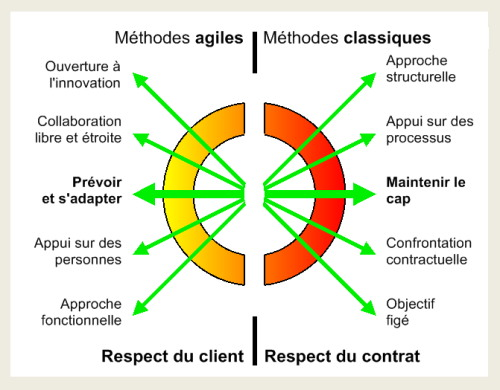
\includegraphics[width=0.6\linewidth, height=6.7cm]{images/comparaison.png}
\caption{Méthode Agile vs Méthode Classique \cite{agilevsclassic2017}}
\label{fig:classique_vs_agile}
\end{figure} 
\newpage 
\subsection{Méthodes agiles}

Après une comparaison des méthodes classiques et agiles, nous avons choisi une approche agile pour sa flexibilité. Une comparaison entre Scrum, Kanban et XP a ensuite été réalisée afin de sélectionner la méthode la plus adaptée à notre projet. 
\begin{longtable}{|p{4cm}|p{4cm}|p{4cm}|p{4cm}|}

\caption{Comparaison des méthodes agiles\cite{agile_comparatif_artza}} \\
\hline

\rowcolor{coloranihub}
\textbf{Critère} & \textbf{Scrum} & \textbf{Kanban} & \textbf{XP (Extreme Programming)} \\
\hline
\endfirsthead

\hline
\rowcolor{coloranihub}
\textbf{Critère} & \textbf{Scrum} & \textbf{Kanban} & \textbf{XP (Extreme Programming)} \\
\hline
\endhead

Organisation du travail & Basée sur des sprints & Flux continu & Itérations courtes \\
\hline

Planification & Fixée au début du sprint & Flexible et continue & Très fréquente et adaptative \\
\hline

Gestion des tâches & Backlog de sprint & Tableau Kanban (To Do / Doing / Done) & User stories détaillées \\
\hline

Rôles définis & Oui (Scrum Master, Product Owner, équipe) & Non obligatoire & Oui mais moins formalisés \\
\hline

Changement des exigences & Limité pendant le sprint & Accepté à tout moment & Accepté en continu \\
\hline

Livraison & À la fin de chaque sprint & Continue & Très fréquente \\
\hline

Qualité du code & Non spécifique & Non spécifique & Très forte (TDD, pair programming) \\
\hline

Implication client & Élevée à chaque sprint review & Variable & Très élevée et continue \\
\hline

Adapté pour & Projets structurés & Maintenance / flux continu & Projets techniques exigeants \\
\hline

\end{longtable}

\subsection{Méthodologie adoptée : Scrum}

Scrum est un cadre de travail agile permettant de gérer des projets complexes de manière itérative et incrémentale. Il repose sur une organisation structurée favorisant la collaboration, la transparence et l’adaptation continue tout au long du projet \cite{scrum_atlassian} . 
\subsubsection*{Équipe Scrum}

L’équipe Scrum est composée de plusieurs rôles complémentaires \cite{scrum_roles_atlassian} :

\begin{itemize}
    \item \textbf{Product Owner} : responsable de la définition des besoins du client et de la gestion du Product Backlog. Il priorise les fonctionnalités à développer.
    
    \item \textbf{Scrum Master} : garant du respect de la méthodologie Scrum. Il facilite le travail de l’équipe et élimine les obstacles rencontrés.
    
    \item \textbf{Équipe de développement} : composée des développeurs, elle est responsable de la conception, du développement et de la livraison du produit.
\end{itemize}

\subsubsection*{Les événements Scrum}

Scrum s’organise autour de plusieurs événements clés \cite{scrum_ceremonies_atlassian} :

\begin{itemize}
    \item \textbf{Sprint} : période courte (généralement 2 à 4 semaines) durant laquelle une version fonctionnelle du produit est développée.
    
    \item \textbf{Sprint Planning} : réunion de planification au début de chaque sprint pour définir les objectifs et les tâches à réaliser.
    
    \item \textbf{Daily Scrum (Daily Meeting)} : réunion quotidienne courte permettant de suivre l’avancement, identifier les obstacles et synchroniser l’équipe.
    
    \item \textbf{Sprint Review} : réunion en fin de sprint pour présenter les fonctionnalités développées au client et recueillir ses retours.
    
    \item \textbf{Sprint Retrospective} : réunion interne visant à analyser le sprint écoulé et à améliorer les processus de travail.
\end{itemize} 


\subsubsection*{Les artefacts Scrum (éléments clés)}

Les artefacts Scrum représentent les éléments essentiels du suivi du projet \cite{scrum_artifacts_atlassian} :

\begin{itemize}
    \item \textbf{Product Backlog} : liste priorisée de toutes les fonctionnalités et exigences du projet.
    
    \item \textbf{Sprint Backlog} : ensemble des tâches sélectionnées pour être réalisées durant un sprint.
    
    \item \textbf{Increment (Incrément)} : version fonctionnelle du produit livrée à la fin de chaque sprint, intégrant les nouvelles fonctionnalités développées.
\end{itemize} 
\subsubsection{Processus Scrum} 
La figure \ref{fig:scrum_process} illustre le processus de travail de Scrum , mettant en évidence les différentes étapes et interactions entre les rôles, les événements et les artefacts tout au long du projet : 
\begin{figure}[H]
\centering
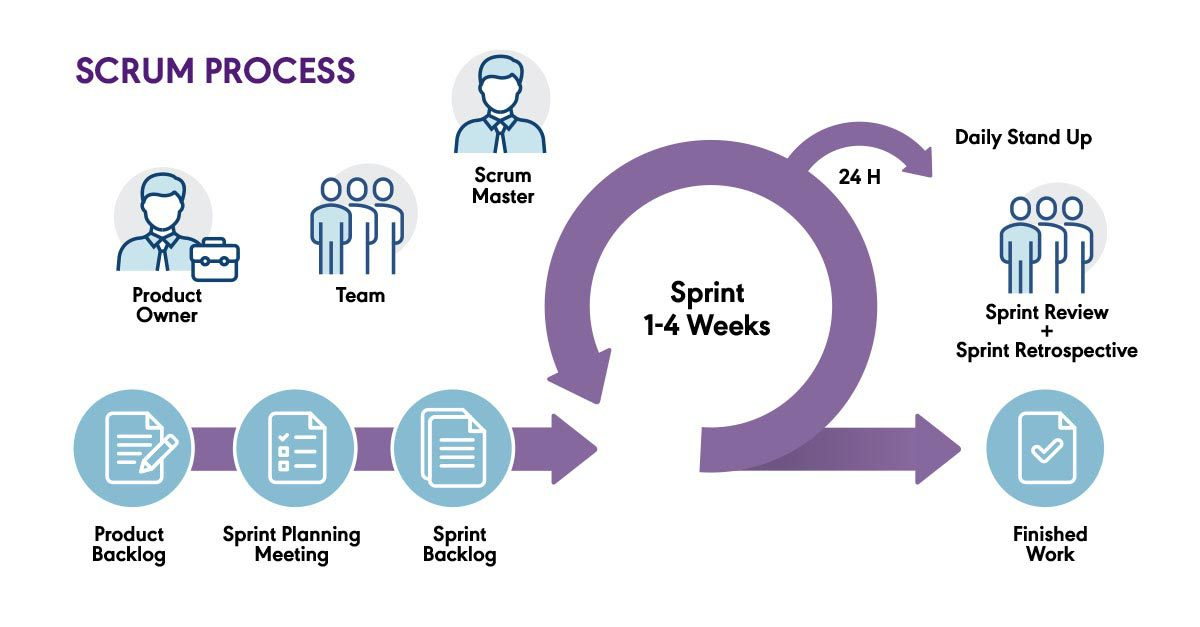
\includegraphics[width=0.9\linewidth, height=7cm]{images/scrum.jpg}
\caption{Processus de travail de Scrum \cite{scrum_process_pm}}
\label{fig:scrum_process}
\end{figure}  
Dans le cadre de notre projet, nous avons opté pour une planification basée sur la méthodologie Scrum, en définissant \textbf{6 sprints} répartis en \textbf{2 releases}. Cette organisation permet une progression incrémentale du développement, ainsi qu’une meilleure maîtrise des fonctionnalités livrées à chaque étape. Nous décrirons cette décomposition en détail à la fin du chapitre deux, après avoir présenté et défini l’ensemble des fonctionnalités du produit à réaliser.
\newpage 





\section{Chronogramme} 
La figure ci-dessous présente les différentes étapes de réalisation de notre projet, planifiées sur une période de stage de 4 mois, s’étendant du 1er février 2026 au 31 mai 2026.
\begin{figure*}[ht]
\centering
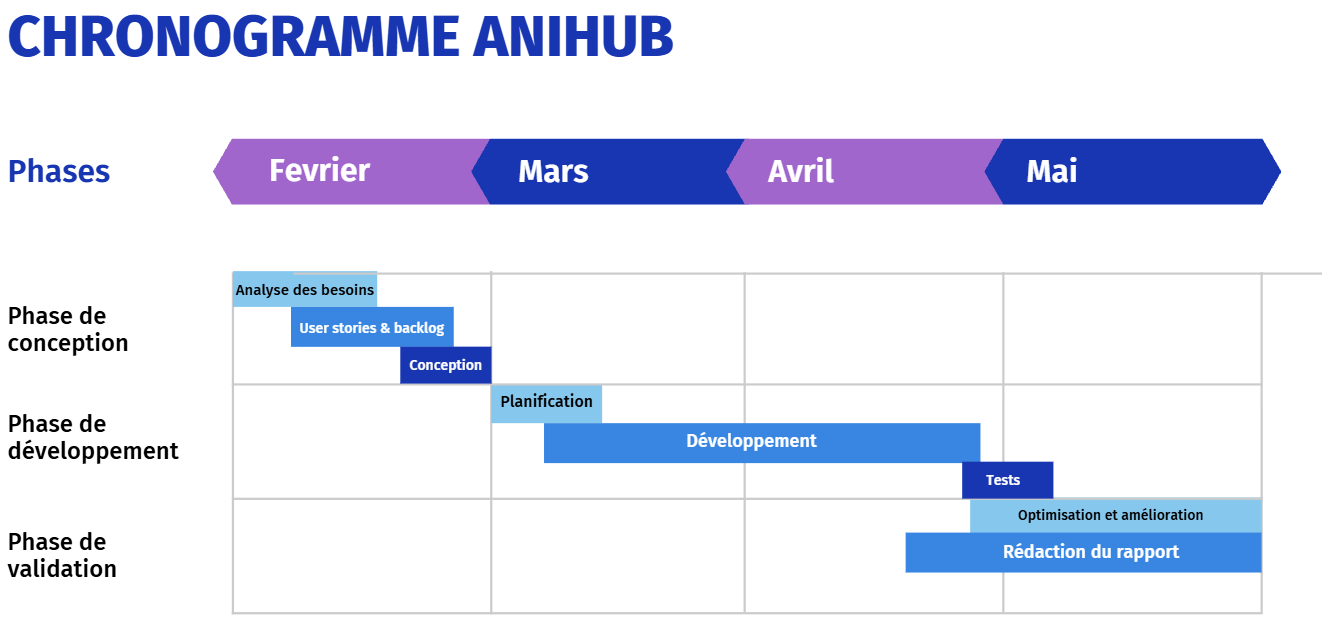
\includegraphics[width=0.95\linewidth, height=8cm]{images/chronogramme.png}
\caption{Chronogramme AniHub}
\label{fig:image}
\end{figure*}  

\section{Conclusion}

Dans ce chapitre, nous avons présenté le cadre général du projet AniHub ainsi que l’organisme d’accueil, AfterCode. Nous avons également réalisé une analyse de l’existant afin d’identifier les limites des solutions actuelles du marché des animaux domestiques en Tunisie. Sur cette base, nous avons proposé notre solution en détaillant ses principaux modules ainsi que ses objectifs et son positionnement stratégique. Enfin, nous avons introduit la méthodologie de développement adoptée, basée sur Scrum, qui structure le projet en plusieurs sprints et releases afin d’assurer un développement progressif et maîtrisé.